% !TEX root = algo-quicksheet.tex
\chapter{Array}
\section{Two-pointer Algorithm}
\runinhead{Container With Most Water.} Given coordinate $(i, a_i)$, find two lines, which together with x-axis forms a container, such that the container contains the most water.
\begin{figure}[hbtp]
\centering
\subfloat{\includegraphics[width=0.8\linewidth]{Container-With-Most-Water.jpg}}
\caption{Container with Most Water}
\label{fig:Container-With-Most-Water}
\end{figure}

When calculate water area, the water height $h$ is constrained by $\min(h_{lo}, h_{hi})$. Core clues:
\begin{enumerate}
\item \textbf{Extreme cases}: start from the extreme cases $\Ra$ be greedy.
\item \textbf{Two pointers}: Two pointers $lo$, $hi$ at two ends, calculate the current area.
\item \textbf{Move one}: Move the shorter (lower height) pointer. 
\end{enumerate}

Why does this greedy algorithm work? When searching further, we always search the best one.  When searching the most-water container with length $l$, we always reach the maximum area. When shrinking the water length by 1, we always reach the higher height. 

If we don't drop the lower side, we will always be constrained by the lower side. 

\runinhead{Minimum Window Substring.} Given two strings $s$ and $t$ respectively, return the minimum window substring of $s$ such that every character in $t$ (including duplicates) is included in the window.
\begin{python}
Input: s = "ADOBECODEBANC", t = "ABC"
Output: "BANC"
\end{python}

\rih{Core Clues:}
\begin{enumerate}
\item Window $\Ra$ sliding window, two pointers
\item Check whether cover $t$ with duplicates $\Ra$ dictionary
\item Whether full match $\Ra$ counter of missing or matched
\end{enumerate}
\begin{python}
def minWindow(s, t):
  N = len(s)
  requires = defaultdict(int)
  for ch in t:
    requires[ch] += 1

  missing = len(t)
  lo = 0
  start = 0
  end = len(s)
  for i in range(N):
    ch = s[i]
    if ch in requires:
      if requires[ch] > 0:
        missing -= 1
      requires[ch] -= 1

    # when full matched
    if missing == 0:
      hi = i + 1
      while lo < hi:
        if s[lo] in requires: 
          if requires[s[lo]] < 0:
            requires[s[lo]] += 1
          else:
            break

        lo += 1

      # update best window
      if hi - lo < end - start:
        start, end = lo, hi
      
      # since found, move left to search for next valid window
      if s[lo] in requires:
        requires[s[lo]] += 1
        missing += 1
      lo += 1

  return s[start:end]
\end{python}
\subsection{Interleaving}
\runinhead{Interleaving positive and negative numbers.} Given an array with positive and negative integers. Re-range it to interleaving with positive and negative integers.
\begin{lstlisting}
Input:
[-33, -19, 30, 26, 21, -9]
Output:
[-33, 30, -19, 26, -9, 21]
\end{lstlisting}
Core clues:
\begin{enumerate}
\item How to do it in O(N).
\item What (positive or negative) is expected for the current position.
\item Where is the next positive and negative element.
\end{enumerate}
\begin{python}
def rearrange(self, A):
    n = len(A)
    pos_cnt = len(filter(lambda x: x > 0, A))
    pos_expt = True if pos_cnt * 2 > n else False

    neg = 0  # next negative
    pos = 0  # next positive
    for i in range(n):
        # search for the next 
        while neg < n and A[neg] > 0:
            neg += 1
        while pos < n and A[pos] < 0:
            pos += 1
        
        if pos_expt:
            A[i], A[pos] = A[pos], A[i]
        else:
            A[i], A[neg] = A[neg], A[i]
        
        pos_expt = not pos_expt
        
        # handle same-idx swap
        if i == neg:
            neg += 1
        if i == pos:
            pos += 1
\end{python}

\section{Circular Array}
This section describes common patterns for solving problems with circular arrays.

Normally, we should solve the linear problem and circular problem very differently.

\subsection{Circular max sum}
Linear (acyclic) problem can be solved linear with DP algorithm for maximum subarray sum - Section \ref{dpSequence}. 

The circular sum should use dp. 

Problem description: Given an integer array containing both positive and negative, find a continuous rotate subarray where the sum of numbers is the largest. Return the index of the first number and the index of the last number. 
\runinhead{Core clues:}
\begin{enumerate}
\item \textbf{State definitions}: 

\rih{Max subarray sum from index 0}. Construct left max sum $L_i$ for max sum over the $A[:i]$ with subarray starting at 0 (\textit{forward} starting from the left side), up to $A_{i-1}$. 

\rih{Max subarray sum from index -1}. Construct right max sum $R_i$ for max sum over the indexes $A[i:]$, with subarray ending at -1 (\textit{backward} starting from the right side), up to $A_i$. 

\item \textbf{Transition functions:}
\begin{align*}
L_i = \max\Big(L_{i-1}, sum(A[:i])\Big) \\ 
R_i = \max\Big(R_{i+1}, sum(A[i:])\Big)
\end{align*}

\item \textbf{Global result}: 
$$maxa = \max(R_i+L_i, \forall i)$$
\end{enumerate}

\subsection{Non-adjacent cell}
Maximum sum of non-adjacent cells in a circular array $A$. (House robbery problem)

Relax to linear problem, non-circular array. We need to consider the decision on $A_i$. 
\begin{enumerate}
\item Take the $A_i$
\item Not take the $A_i$ 
\end{enumerate}
The transition funciton is:
\begin{align*}
F_{i} = \max\big(F_{i-1}, F_{i-2}+A_{i-2}\big)
\end{align*}
Linear \ref{dpSequence}. 

To solve it in circular array, either 
\begin{itemize}
\item Include $A_0$ and exlcude $A_{-1}$ or 
\item Include $A_{-1}$ and exclude $A_0$.
\end{itemize}
\begin{python}
def rob(self, A):
    n = len(A)
    if n <= 1:
        return sum(A)

    # ignore A[~0]
    F = [0] * (n+2)  # two dummy states F_0, F_1
    for i in range(2, 2 + n - 1):
        F[i] = max(F[i-1], F[i-2] + A[i-2])
    
    ret = F[~1]  # not F[~0]

    # ignore A[0]
    F = [0] * (n+2)
    for i in range(2 + 1, 2 + n):
        F[i] =  max(F[i-1], F[i-2] + A[i-2])
    
    ret = max(ret, F[~0])
    return ret
\end{python}


\subsection{Binary search}
Searching for an element in a circular sorted array. Half of the array is sorted while the other half is not.
\begin{python}
A = [1, 2, 3, 4, 5, 6, 7]
B = [4, 5, 6, 7, 1, 2, 3]
\end{python}
\begin{enumerate}
\item If $A_0 < A_{mid}$, then all values in the first half of the array are sorted.
\item If $A_{mid} < A_{\sim 0}$, then all values in the second half of the array are sorted.
\item Then \textit{derive and decide} whether to got the \textbf{sorted half} or the \textbf{unsorted half}.
\end{enumerate}

\section{Local Search - Monotonic Stack}\label{monostack}
\subsection{Next/Prev Smaller Value}\label{allNearestSmaller}

\textbf{Previous Smaller Element}. Left / previous neighbor of a value $v$ to be the value that occurs prior to $v$, is smaller than $v$, and is closer in position to $v$ than any other smaller value.

\rih{Core clues:}
\begin{enumerate}
\item Nearest $\equiv$ spatial locality.
\item \textbf{Search Backward}: for each position in a sequence of numbers, search among the \textit{previous} positions for the last position that contains a smaller value. 
\item \textbf{Invariant}: Maintain a \textit{motonotically increasing} stack.  
\item If the question asks for all nearest \textit{larger} values, maintain a \textit{motonotically decreasing} stack.  
\end{enumerate}

\begin{python}
def prev_smaller_item(self, A):
    N = len(A)
    L = [-1 for _ in A]
    stk = []
    for i in range(N):
        while stk and A[stk[-1]] >= A[i]:
            stk.pop()

        if stk:
            L[i] = stk[-1]
            
        stk.append(i)  # store the idx

    return L
\end{python}

\runinhead{Next smaller Element  - Mirrored Problem.} For each item in the array $A$, find the next cloest smaller item. 

\rih{Core Clues}:
\begin{enumerate}
\item Search forward: inituitively when we scan the current index $i$, we want to find the next cloeset index $j$ that satifies the condition. However, we cannot store the candidates $j$'s in some data structure to reduce time complexity from $O(N^2)$ of brute force. 
\item \rih{Match backward}: hold previous items in some data structure, and efficient match the previous element when $A_{prev} > A_{cur}$.
\item Monotonic stack: use a monotonic stack to remember the previous items that are pending to find a smaller element in the future. It is a monotonic increasing stack from left to right in this case. 
\item Resolve the previous pending items: when current index $i$ has a smaller value than the previous items, we resolve the previous items as we have found the next closest smaller item as $i$ for them, by popping the stack. 
\item Alternatively, we can scan from right to left to reduce to previous smaller element. 
\end{enumerate}
The monotonic stack holds pending items that have not found the next smaller element, untill the monotonicity is broken by the current scanning element $A_i$. We pop the previous pending items and resolve their next smaller element as $A_i$. 

\begin{python}
def next_smaller_item(A):
    N = len(A)
    # next item on the right
    R = [-1 for _ in range(N)]
    # store the previous, mono asc stk
    stk = [] 
    
    for i in range(N):
        while stk and A[stk[-1]] >= A[i]:
            prev = stk.pop()
            R[prev] = i  # found
        stk.append(i)
    
    return R
\end{python}

\runinhead{Largest Mountain.} Find the largest mountain area in the histogram. Given $N$ non-negative integers $H$ representing the histogram's bar height where the width of each bar is 1, find the area of largest mountain. 

We are to remove some bricks from the bar to form a mountain-shaped arrangement. In this arrangement, the tower heights are non-decreasing, reaching a maximum peak value with one or multiple consecutive towers and then non-increasing. For example, $H = [6,5,3,9,2,7]$ bececomes $[3,3,3,9,2,2]$ with the largest area of 22.

\rih{Core Clues:}
\begin{enumerate}
\item DP: let $L_i$ be the largest asc slide area for \pyinline{H[:i]}, peaked at $H_{i-1}$, scanning from left to right. Let $R_i$ be the largest desc slide area for \pyinline{H[i:]}, peaked at $H_i$, scanning from right to left. 
\item Previous smaller element: When processing $H_i$, define $lo$ as the previous smaller element for $H_i$ on the left
\[
    L_{i+1} =+
    \begin{cases}
        L_{prev+1} & \text{for range }[0,prev]\\
        (i-prev) * H_{i} &\text{for range }(prev, i]
    \end{cases}
\]
Substitute $i$ with $i-1$, 
\[
    L_{i} =+
    \begin{cases}
        L_{prev+1} & \text{for range }[0,prev]\\
        (i-1-prev) * H_{i-1} &\text{for range }(prev, i-1]
    \end{cases}
\]

\item Mono stack: use monotononically increasing stack to find the previous smaller item on the left. 
\item Reverse then reverse back: for $R_i$, we can reuse the same logic, but since it is from right to left, we need to revere $H$ to get $R$, and then reverse $R$ back.
\end{enumerate}
\begin{python}
def largest_mountain_area(self, H):
    N = len(H)
    L = self.dp(H)
    R = self.dp(H[::-1])[::-1] # reverse then reverse back
    
    maxa = 0
    for i in range(N+1):
    	# H[:i] & H[i:]
        cur = L[i] + R[i]
        maxa = max(maxa, cur)

    return maxa

def dp(self, H):
    N = len(H)
    L = [0 for _ in range(N+1)]
    stk = []  # mono asc
    for i in range(1, N+1):
        idx = i-1
        while stk and H[stk[-1]] > H[idx]:
            stk.pop()
            
        prev = stk[-1] if stk else -1
        # [0, prev] and (prev, idx]
        L[i] = L[prev+1] + (idx-prev) * H[idx] 
        stk.append(idx)
    
    return L
\end{python}

\subsection{Local Minimum/Maximum}
\begin{itemize}
\item To find the boundaries for \textbf{local max} of $A_{mid}$ as $(lo, i$):
$$
A_{lo} > A_{mid} < A_{i}
$$
$\La$ maintain a monotonically \textbf{decreasing} stack. \ 

\item To find the boundaries for \textbf{local min} of $A_{mid}$ as $(lo, i)$:
$$
A_{lo} < A_{mid} > A_{i}
$$
$\La$ maintain a monotonically \textbf{increasing} stack. 
\item The boundary is $(lo, i)$: $(lo, mid], [mid, i)$.
\end{itemize}

\runinhead{Minimize Cost of Merging Subarray.} We have an array $A$ of positive integers. We must repeatedly merge two adjacent subarray into one, starting from 1-element subarray. The cost of merging two subarrays is the product of their largest elements. Determine the total cost to merge everything into one subarray.

\rih{Core Clues:}
\begin{enumerate}
\item Cost: To remove any number $a$, it costs $a * b$, where $b \geq a$. So $a$ has to be removed by a bigger neighbor $b$. To minimize this cost, we need to minimize $b$.
\item Greedy: Max element is used at each subarray $\Ra$ put big leaf nodes closer to the top/root $\Ra$ greedily start with the smallest leaf.
\item Everytime the smaller element is merged, it is gone. Brute:
\begin{python}
i = A.index(min(A))
cost += A[i] * min(A[i-1], A[i+1])
A.pop(i)
\end{python}
This is $O(N^2)$. 
\item Merging is a local event. Find local min: we need to find $i$ s.t. 
$$A_{lo} > A_{mid} < A_i$$
$\La$ keep a monotonic decreasing stack for $A_{0:i}$, till the monotonicity is broken by $A_i$, then we need to pop the stack and maintain the monotonicity. 
\item $A_{mid}$ is merged. The mono stack is holding the unmerged items on the left side.
\end{enumerate}

\begin{python}
def min_cost_merging_leaf_values(A):
    cost = 0
    stk = []
    for a in A:
        while stk and stk[-1] <= a:
            mid = stk.pop()
            # merging mid
            if stk:
                left = stk[-1]
                cost += mid * min(left, a)
            else:
                cost += mid * a
                
        stk.append(a)
    
    # can append sys.maxsize as sentiel to flush 
    while len(stk) > 1:
        mid = stk.pop()
        left = stk[-1]
        cost += mid * left
    
    return cost
\end{python}

\runinhead{Sum of All Subarray Ranges.} A subarray range is defined as $\max - \min$. Find the sum of subarray ranges for all subarrays. 

\rih{Core Clues:}
\begin{enumerate}
\item To get the range: get the min and max. To get all subarrays: iterate i and j, keep tracks of min and max. Thus $O(N^2)$.
\item We transform the range sums:
\[
\begin{aligned}
&\sum{range} \\
&=\sum{(\max-\min)} \\
&=\sum{\max} - \sum{\min}
\end{aligned}
\]
\item To get $\sum{\max}$: \#times as local min $\times$ val. 
\item To get the \textbf{bounds} for local min: 
$$A_{lo} < A_{mid} > A_i$$ 
$\La$ use monotonically increasing stack.
\item The number of subarrays centered at $A_{mid}$: $|(lo, mid]| \times |[mid, i)|$.
\item Similarly, find the \textbf{bounds} for local max:
$$A_{lo} > A_{mid} < A_i$$ 
\end{enumerate}
\begin{python}
def subarray_ranges(self, A):
    N = len(A)
    ret = 0

    sum_max = 0
    stk = []  # mono desc stk for local max
    A.append(sys.maxsize)
    for i in range(N+1):
        while stk and A[stk[-1]] < A[i]:
            mid = stk.pop()
            lo = stk[-1] if stk else -1
            # times: [mid, i), (lo, mid]
            cnt = (i - mid) * (mid - lo)
            sum_max += cnt * A[mid]
        stk.append(i)
    A.pop()

    sum_min = 0
    stk = []  # mono asc stk for local min
    A.append(-sys.maxsize-1)
    for i in range(N+1):
        while stk and A[stk[-1]] > A[i]:
            mid = stk.pop()
            lo = stk[-1] if stk else -1
            # times: [mid, i), (lo, mid]
            cnt = (i-mid) * (mid - lo)
            sum_min += cnt * A[mid]
        stk.append(i)
    A.pop()
    
    return sum_max - sum_min
\end{python}

\runinhead{Largest Rectangle.} Find the largest rectangle in the matrix (histogram). Given $n$ non-negative integers representing the histogram's bar height where the width of each bar is 1, find the area of largest rectangle in the histogram. 

\begin{figure}[]
\centering
\subfloat{\includegraphics[width=0.4\linewidth]{histogram_area}}
\caption{Largest rectangle in histogram\\ $i \ra$ height 2, $cur \ra$ height 6, 5, 1}
\label{fig:histogram_area}
\end{figure}

\rih{Core clues:}
\begin{enumerate}
\item Largest rectangle: when scanning index $i$, calculate the rectangle area with a height $h$ s.t. $h > H_i$. We want to find the leargest rectangle in \pyinline{H[lo:i]}. 
\item \rih{Local min}: the rectangle area is calcualted as local min height $\times$ its range. To find the boundaries for local min of $A_{mid}$ as $(lo, i$). $H$ and $A$ are interchangeable:
$$
A_{lo} < A_{mid} > A_{i}
$$
\item Monotonic stack: maintain the monotonic increasing (non-decreasing) stack, with increasing indices with scanning $i$. 
\item Post-processing in the end
\end{enumerate}

Code:
\begin{python}
def largest_rectangle_area(self, H):
    N = len(H)
    maxa = -sys.maxsize-1
    stk = []  # store the idx, mono asc stack
	
    H.append(-sys.maxsize-1)  # sentiel to flush
    for i in range(N+1):
        while stk and H[stk[-1]] > H[i]:
            mid = stk.pop()
            # calculate area when popping
            # bound: (lo, i), [lo+1, i)
            lo = stk[-1] if stk else -1
            l = i - (lo+1)
            area = H[mid]*l
            maxa = max(maxa, area)

        stk.append(i)
    H.pop()  # clear

    return maxa
\end{python}
Maintain a monotonic stack to store the bars in non-decreasing, then calculate the area by popping out the stack to get the currently lowest bar which determines the height of the rectangle.
\begin{itemize}
\item Height: on the left side of $h$, all the higher heights than $h$ are popped thus absent; while on the right side of $h$, all have higher heights until $H_i$. 
\item Width: 1) what are \textbf{not in} the stack have higher heights than $h$; and 2) the earlier elements \textbf{in} the stack have smaller heights than $h$, $\Ra$ the lower bound is $lo = stk_{-1}+1$.
\end{itemize}
\begin{figure}[]
\centering
\subfloat{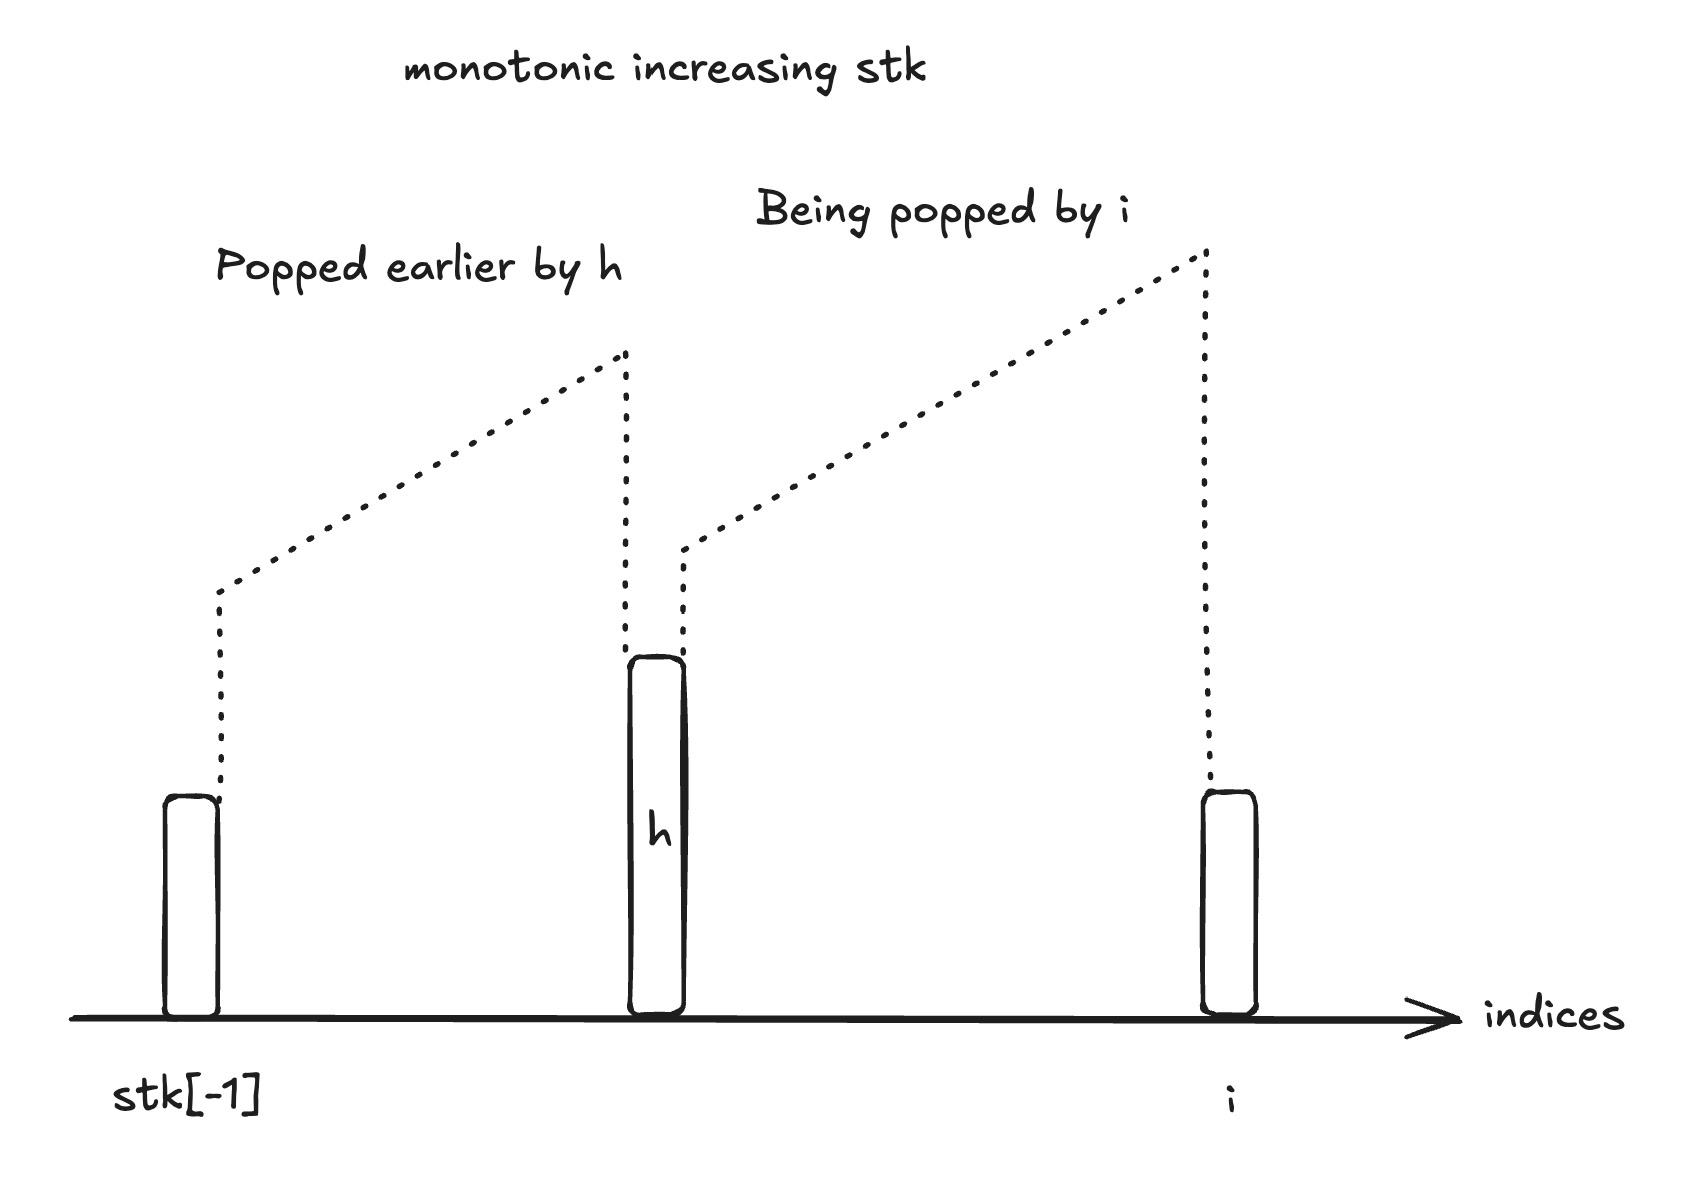
\includegraphics[width=1\linewidth]{monotonic_stk}}
\caption{Monotonic stack before and after $h$}
\label{fig:monotonic_stk}
\end{figure}

\subsection{Monotonic Greedy Search}
\runinhead{Lexically Smallest Distinct-Element Subsequence.} Given a string $s$, return the lexicographically smallest subsequence of $s$ that contains all the distinct characters of $s$ exactly once. For example, \pyinline{s = "cbacdcbc"}, return \pyinline{"acdb"}. \pyinline{s = "cba"}, return \pyinline{"cba"}

\rih{Core Clues:}
\begin{enumerate}
\item Greedy goal: smallest $\Ra$ always place smaller chars earlier if possible to get the lexicographically smallest result.
\item Contains all the distinct chars of $s$ exactly once $\Ra$ \pyinline{visited}
\item Monotonic stack: maintain a stack where chars are as lexicographically small as possible in stack by popping bigger chars if they can reappear later.
\item Last occurrence check: to ensure the result contain all distinct chars $\Ra$ before popping a char from the stack, ensure it appears again later.
\end{enumerate}
\begin{python}
def smallest_subsequence(s):
    stk = []
    last_occur = defaultdict(int)
    for i, c in enumerate(s):
        last_occur[c] = i
    
    visited = defaultdict(bool)
    for i, c in enumerate(s):
        if not visited[c]:
            while stk and stk[~0] > c \
                and last_occur[stk[~0]] > i:
                e = stk.pop()
                visited[e] = False

            stk.append(c)
            visited[c] = True
    
    return "".join(stk)
\end{python}


\runinhead{Longest Positive Subarray Sum.} Given a list $A$ of numbers, find the longest positive subarray sum. 

\rih{Core Clues}:
\begin{enumerate}
\item Subarray sum $\Ra$ prefix sum.
\item Longest positive subarray sum $\slashed{\Ra}$ for $A_i$, find the previous smaller prefix sum 
\item Longest positive subarray sum $\Ra$ 
  \begin{itemize}
  \item Smaller previous index $\Ra$ more potential to be longest 
  \item Smaller prefix sum $\Ra$ more potential to be positive
  \end{itemize}
For $A_i$, the larger previous index is a candidate only because it is having a smaller prefix sum, otherwise there is a smaller index before it for a better potential for find the longest. 

\item Monotonic stack: maintain a value monotonically decreasing stack with increasing indices. The larger indices are put into stack only because it is having a smaller prefix sum. 
\item Greedy longest length: greedily scan $j=i$ from end, and pop the stack until the smallest $j$. 
\end{enumerate}

Correctness of Greedy $\La$ strictly better: 
\begin{enumerate}
\item Scanning form the left, for the same $j$, if $i < i'$, we still need to check $i'$ if its prefix sum is smaller because $i'$ is a valid candidate for the longest positive subarray sum. 
\item Scanning from the right, for the same $j$, if $i > i'$, there is no need to check $(j, i')$ since we have already checked $(j, i)$ which is longer. We have to check a smaller $j'$ for $i'$ to find the longest candidate. 
\end{enumerate}
\begin{python}
def longest_positive_subarray_sum(A):
    N = len(A)
    # prefix sum for A[:i]
    P = [0 for _ in range(N+1)]
    for i in range(1, N+1):
        P[i] = P[i-1] + A[i-1]

    stk = []  # mono desc stack
    for i in range(N+1):
        if not stk or P[stk[~0]] > P[i]:
            stk.append(i)  # greedy
    
    ret = 0
    for i in range(N, 0, -1):
        while stk and P[i] - P[stk[~0]] > 0:
            j = stk.pop()
            ret = max(ret, i - j)
    
    return ret
\end{python}

\section{Sliding Window - Monotonic Queue}\label{monoqueue}
\subsection{Sliding Window}
Typically applied in sliding window. 

\runinhead{Sliding Window Maximum.} Given an array $A$, Find the list of maximum in the sliding window of size $k$ which is moving from the very left of the array to the very right. $\Ra$ mono queue.

Invariant: the queue is storing the non-decreasing-ordered elements of current window.

We want to keep track of the max in sliding window \pyinline{A[i:j+1]} in $O(1)$. Consider a queue $q$ to only store max element at $q_0$. When expanding the window by $j$, if \textbf{trailing} $A_j$ is \textbf{the largest}, we put it at $q_0$, if it is \textbf{second largest}, we put it $q_1$. Similarly for the \textbf{third largest} at $q_2$.  When shrinking the window by $i$, if $q_0$ fall out of the window, we need to promote $q_1$ as the largest. 

If processing a current element $A_j$ to the queue, and the back of the queue has some element smaller than or equal to $A_j$, that smaller element will never be the maximum again once $A_j$ is in the window. Because \textbf{trailing} $A_j$ \textbf{dominates} it (strictly better), and they both sit in the queue.

Now the queue is always in strictly decreasing order from front to back. The front is the largest element. $\blacksquare$

\runinhead{Count Number of Subarrays.} Count number of continuous subarrays in $A$ s.t. within the subarray $|A_i - A_j| \leq 2, \forall i, j$.
\runinhead{Core clues:}
\begin{enumerate}
\item Need to maintain max and min in the sliding window $\Ra$ Monotonic Queue
\item \pyinline{q_min} is monotonically increasing
\item \pyinline{q_max} is monotonically decreasing
\item \pyinline{q_min} and \pyinline{q_max} are storing the indices. 
\end{enumerate}
\begin{python}
def continuous_subarrays(self, A):
    q_max = deque()  # mono desc
    q_min = deque()  # mono asc
    i = 0
    j = 0
    ret = 0
    while j < len(A):
        # process A[j]
        while q_max and A[q_max[~0]] <= A[j]:
            q_max.pop()
        q_max.append(j)
        while q_min and A[q_min[~0]] >= A[j]:
            q_min.pop()
        q_min.append(j)
        
        while q_max and q_min \
            and A[q_max[0]] - A[q_min[0]] > 2:
            # shrink to pass the breaking idx
            prev = q_max.popleft() \
                if q_max[0] < q_min[0] \
                else q_min.popleft()
            i = prev + 1
        
        ret += j - i + 1
        j += 1
        
    return ret 
\end{python}

\runinhead{Longest Subarray With Absolute Diff Less Than or Equal to Limit}. Given an array of integers $A$, and an integer $limit$, return the size of the longest non-empty subarray such that the absolute difference between any two elements of this subarray is less than or equal to limit.

\rih{Core Clues}:
\begin{enumerate}
\item Keep tracks the max and min the sliding window $\Ra$ monotonic queue
\end{enumerate}
\begin{python}
def longestSubarray(self, A, limit) -> int:
  # q_max mono decreasing, front is window max
  # q_min mono increasing, front is window min
  q_max, q_min = deque(), deque()
  ret = 0
  i = 0

  for j in range(len(A)):
    while q_max and A[q_max[~0]] < A[j]:
      q_max.pop()
    q_max.append(j)

    while q_min and A[q_min[~0]] > A[j]:
      q_min.pop()
    q_min.append(j)

    while q_max and q_min \
        and A[q_max[0]] - A[q_min[0]] > limit:
      # move lo up and evict stale indices
      if q_max[0] == i:
        q_max.popleft()
      if q_min[0] == i:
        q_min.popleft()
      i += 1

    ret = max(ret, j - i + 1)

  return ret
\end{python}


\section{Matrix}
\runinhead{Diagonal Traverse}. 
\begin{figure}[hbtp]
\centering
\subfloat{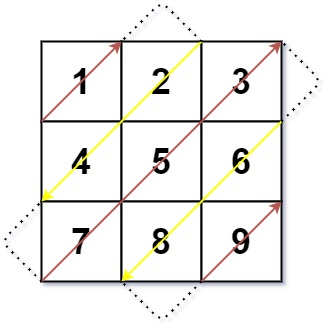
\includegraphics[height=1.2in]{diag1-grid}}
\caption{Diagonal Traverse}
\label{fig:diag1-grid}
\end{figure}
\runinhead{Core Clues}:
Matrix by index
$$
\left[\begin{array}{ccc}
A_{0,0} & A_{0,1} & A_{0,2} \\
A_{1,0} & A_{1,1} & A_{1,2} \\
A_{2,0} & A_{2,1} & A_{2,2}
\end{array}\right]
$$
\begin{enumerate}
\item Diagonal $\Ra r + c = \kappa$ where $\kappa$ is a constant. 
\item Order $Ra$ $\kappa$ determines the order of elements within a diagonal.
\end{enumerate}
\begin{python}
def findDiagonalOrder(self, matrix):
    R, C = len(matrix), len(matrix[0])
    F = [[] for _ in range((R-1)+(C-1)+1)]
    for r in range(R):
        for c in range(C):
            F[r+c].append(matrix[r][c])

    ret = []
    for i in range(R+C-1):
        if i % 2 == 1:
            ret.extend(F[i])
        else:
            ret.extend(F[i][::-1])

    return ret
\end{python}
\section{Voting Algorithm}
\subsection{Majority Number}
\subsubsection{$\frac{1}{2}$ of the Size}
Given an array of integers, the majority number is the number that occurs more than half of the size of the array. 

Algorithm: Majority Vote Algorithm. Maintain a counter to count how many times the majority number appear more than any other elements before index $i$ and after re-initialization. Re-initialization happens when the counter drops to 0. 

Proof: Find majority number $x$ in $A$. Mathematically, find $x$ in array $A$ with length $n$ s.t. $cnt_x > n -cnt_x$. 

Find a \textbf{pair} $(a_i, a_j)$ in $A$, if $a_i \neq a_j$, delete both from $A$. The counter  still
holds that: $C^{A'}_x > |A'|-C^{A'}_x$. Proof, since $a_i\neq a_j$, at most 1 of them
equals $x$, then $C^{A'}_x$ decrements at most by 1, $|A'|$ decrements by 2.

To find such pair $(a_i, a_j), a_i\neq a_j$, linear time one-pass algorithm. That's
why \textit{Moore's voting algorithm} is correct.

At any time in the execution, let $A'$ be the prefix of $A$ that has been processed,
if $counter>0$, then keep track the candidate $x$'s counter, the $x$
is the majority number of $A'$.  If $counter =0$, then for $A'$ we can pair the elements
s.t. are all pairs has distinct element. Thus, it does not hold that $cnt_x>n-cnt_x$;
thus $x\in A'$. $\blacksquare$
 
Re-check: This algorithm needs to re-check the current number being counted is indeed the majority number.    

\begin{python}
def majorityElement(self, nums):
    """
    Algorithm:
    O(n lgn) sort and take the middle one
    O(n) Moore's Voting Algorithm
    """
    mjr = nums[0]
    cnt = 0
    for i, v in enumerate(nums):
        if mjr == v:
            cnt += 1
        else:
            cnt -= 1

        if cnt < 0:
            mjr = v
            cnt = 1

    return mjr

\end{python}
\subsubsection{$\frac{1}{3}$ of the Size}
Given an array of integers, the majority number is the number that occurs more than $\frac{1}{3}$ of the size of the array. This question can be generalized to be solved by $\frac{1}{k}$ case. 

\subsubsection{$\frac{1}{k}$ of the Size}
Given an array of integers and a number k, the majority number is the number that occurs more than $\frac{1}{k}$ of the size of the array. In this case, we need to generalize the solution to $\frac{1}{2}$ majority number problem.

\begin{python}

def majorityNumber(self, A, k):
    """
    Since majority elements appears more 
    than ceil(n/k) times, there are at 
    most k-1 majority number
    """
    cnt = defaultdict(int)
    for e in A:
        if e in cnt:
            cnt[e] += 1
        else:
            if len(cnt) < k-1:
                cnt[e] += 1
            else:
                for key in cnt.keys():
                    cnt[key] -= 1
                    if cnt[key] == 0:
                        del cnt[key]
    
    
    # filter, double-check
    for key in cnt.keys():
        if len(filter(lambda x: x == key, A)) 
            > len(A)/k:
            return key

    raise Exception
\end{python}

\section{Index Remapping}
\subsection{Introduction}
\runinhead{Virtual Index.} Similar to physical and virtual machine, the underlying indexing $i$ for an array $A$ is the physical index, while we can create virtual indexing $i'$ for the same array $A$ to map $A_{i'}$ to a physical entry $A_{i}$.
\subsection{Example}
\runinhead{Interleaving indexes} Given an array $A$ of length $N$, we want to mapping the virtual indexes to physical indexes such that $A_0$ maps to $A_1$, $A_1$ maps to $A_3$,..., $A_{\lfloor N/2\rfloor}$ maps to $A_0$, as followed: 
\begin{figure}[hbtp]
\centering
\subfloat{\includegraphics[width=\linewidth]{virtual_indexes.png}}
\caption{Virtual Indices Remapping}
\label{fig:virtual_indexes}
\end{figure}

Find the pattern: 
$$
2*i = p'
$$
\begin{python}
N = 6
v	p`	p
0	1	1
1	3	3
2	5	5
3	7	0
4	9	2
5	11	4

N = 7
v	p`	p
0	1	1
1	3	3
2	5	5
3	7	0
4	9	2
5	11	4
6	13	6

\end{python}
\begin{lstlisting}
0 -> 1
1 -> 3
2 -> 5
...
N/2-1 -> N-1 or N-2

N/2 -> 0
N/2+1 -> 2
...
N -> N-2 or N-1
\end{lstlisting}


If $N$ is even, 

$$
(2*i+1)\%(N+1)
$$

If $N$ is odd,

$$
(2*i+1)\%(N)
$$

Thus, by combining two cases, we create the mapping relationship: 
\begin{python}
def idx(i):
    return (2*i+1) % (N|1)
\end{python}

